\section{Feature engineering}\label{sec:features}

Each feature below has a plain definition, the reason it should help, and the result of removing it (or adding it)
on the five development folds. The removals are made one at a time on the untuned ridge-plus-trees model (ladder
step 5, \usd{\DevStepE}), following the advice to test feature groups against out-of-sample error rather than
importance scores \citep{kuhn2019feature}. Table~\ref{tab:ablations} has every result with its paired interval.

\begin{description}
  \item[Load description.] Smooth curves (cubic B-splines) of log distance, weight and the four pickup and delivery
    coordinates, a weight-at-cap flag, and equipment dummies with Dry Van as the reference. Price per mile falls
    smoothly with distance and varies smoothly with location. Coordinates, unlike city names, also work for cities
    the model has never seen.
  \item[market\_level\_today.] The logarithm of the day's mean market index. Its coefficient is an elasticity: the
    fitted model moves the rate by \ElasticityDay\% for each 1\% change in the day's index. Removing the market
    costs \usd{\AblNoMarket}, the largest single loss.
  \item[market\_deviation\_this\_load.] The load's own log index minus the day's mean (elasticity \ElasticityLoad).
  \item[days\_since\_start.] A linear drift beyond the market, \DriftPerMonth\% per month in the final model.
    Removing it costs \usd{\AblNoTrend}; without it every later window is under-forecast.
  \item[quarter\_end\_progress $\times$ equipment.] Zero on the 1st and one on the last day of March, June,
    September and December; zero in other months. Prices ramp up through these months, most for Flatbed. By the
    last day the final model adds \RampDryVan\% for Dry Van, \RampReefer\% for Reefer and \RampFlatbed\% for
    Flatbed. Removing it costs \usd{\AblNoQuarterEnd}: without it the March and June ramps leak into the drift term
    and the drift overshoots.
  \item[distance\_x\_market.] (log distance $-$ 6.8) $\times$ market\_level\_today: long hauls react a little more
    to the market. Removing it costs \usd{\AblNoDistanceXMarket}.
  \item[Weekday dummies (rejected).] Adding them costs \usd{\AblAddDayOfWeek}. The market index already carries
    the weekly price cycle.
  \item[Residual trees.] The LightGBM stage sees distance, weight, coordinates, equipment and both market features.
    Hiding the market features from it costs \usd{\AblResidualTreesWithoutMarket}.
\end{description}

\begin{table}[H]
  \caption{One change at a time against ladder step 5 (dev folds). Positive change = worse.}\label{tab:ablations}
  \inputtable{ablations}
\end{table}

\begin{figure}[H]
  \centering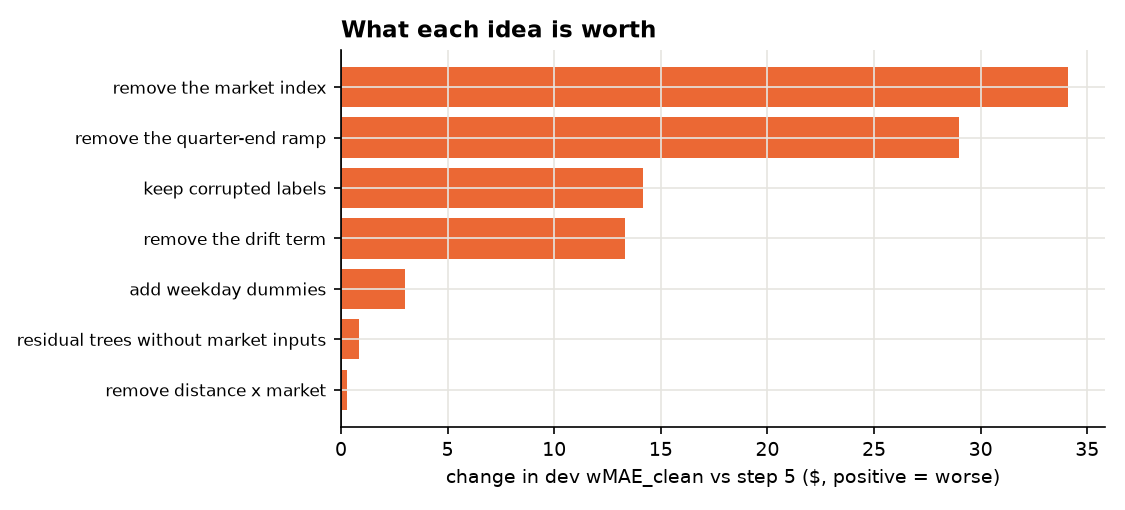
\includegraphics[width=0.8\linewidth]{ablations.png}
  \caption{The same ablations as a chart.}
\end{figure}
